\chapter{Employing GPUs in scientific algorithms}

The information age has brought a massive increase in the amount of data that is being collected and processed. The `data explosion' can be observed in virtually every field of computer science. In the scientific domain, this phenomenon is multiplied by increasingly powerful data-gathering devices (i.e., cytometers in bioinformatics, optic sensors in physics, seismometers in geology, etc.). The amount of data is simply too large to be processed in the required time. In order to alleviate this apparent pressure, the corresponding algorithm (which typically has super-linear time complexity) must be ported to massively parallel architectures, such as GPUs. The provided advantage can result in the ability to assess bigger data, use more detailed processing methods, or analyze the data in real time.

This chapter enumerates four selected scientific algorithms and discusses their challenges in porting to GPUs to enable higher performance.

\section{Hierarchical clustering with the Ma\-ha\-la\-no\-bis linkage}

In the field of bioinformatics, hierarchical clustering is a popular method for analyzing various types of data. 
In general, hierarchical clustering is an unsupervised machine learning method that aims to group the data points into clusters according to some linkage criterion.
It is an iterative method that starts with each data point being a cluster and, in each iteration, merges the two most similar clusters according to the linkage criterion until there is only one cluster.
There are many cluster linkage criteria to choose from, each with advantages and disadvantages. 
The most common linkage is the \emph{centroid linkage}, which computes the distance between the clusters centroids (the mean points).
In analyzing single-cell cytometry data, hierarchical clustering with the Mahalanobis linkage has been shown to be the most suitable method.

Mahalanobis linkage uses \emph{Mahalanobis distance} to measure the similarity between clusters:
\begin{defn}[Mahalanobis distance]
    Suppose a probability distribution $C$ on $\R^d$ with mean $\bar{C} \in \R^d$ and a convariance matrix $\cov(C)$. If the matrix $\cov(C)$ is regular, we define the \emph{Mahalanobis distance} between $u \in \R^d$ and $C$ as
    \begin{equation}
    d_\text{Maha}(u,C) = \sqrt{(u-\bar{C})^T\cov(C)^{-1}(u-\bar{C})}.
    \end{equation}\label{eq01:maha}
\end{defn}

If we generalize a centroid of a cluster to a probability distribution, Definition~\ref{eq01:maha} can be used to define the Mahalanobis distance between a point and a cluster. To extend the definition to a distance between two clusters, we use the following equation:
\begin{equation}
    \delta_\text{Maha}(P,Q) = \frac{d_\text{Maha}(\bar{P},Q) + d_\text{Maha}(\bar{Q},P)}{2}
\end{equation}\label{eq01:maha_linkage}

To illustrate the measure of the Mahalanobis distance, let us suppose we have two elliptic clusters. In the means of the proximity, the measure favors such clusters that their ellipses are alongside rather than in a prolongation of one another [TODO] (see Figure~\ref{fig:ellipses}). 
Only when the objects of a cluster form a spherical shape, this dissimilairity measure is proportional to the Euclidean distance with a corresponding linkage.
This allows for a very natural formation of clusters in biological data. However, the benefits come with the increase in complexity materialized in the computation of covariance matrix, matrix inverse, and vector-matrix-vector multiplication in each distance evaluation.

\begin{figure}[h]
    \centering
    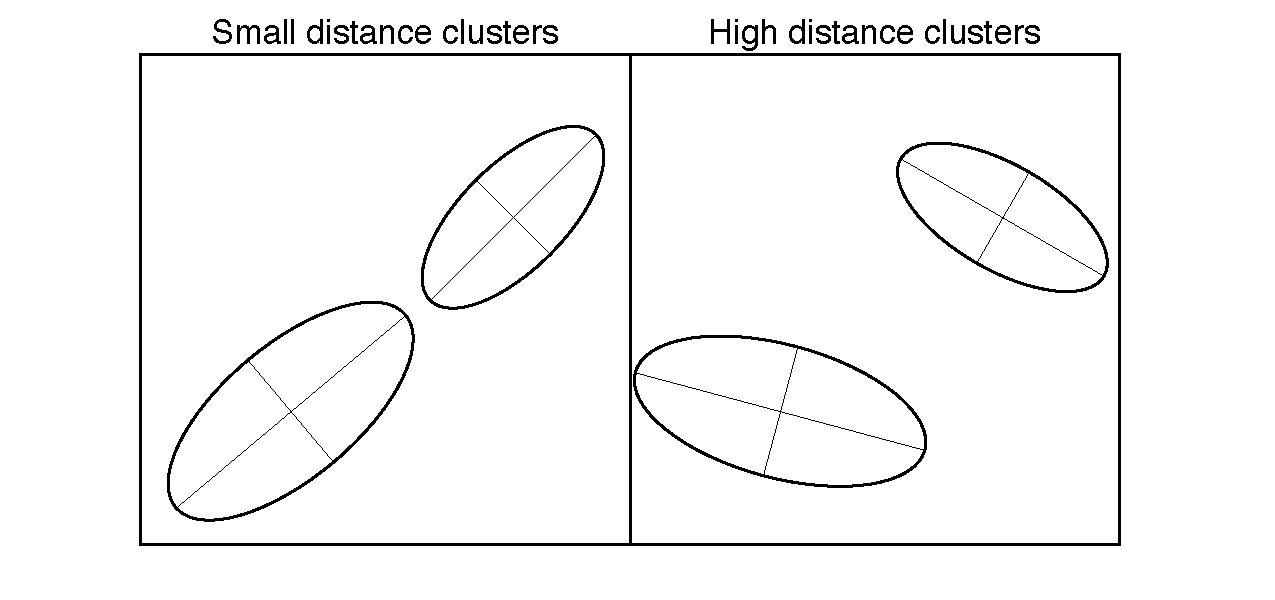
\includegraphics[width=0.6\textwidth]{img/ellipses.pdf}
    \caption{Two pairs of clusters with different similarities according to Mahalanobis distance}
    \label{fig:ellipses}
\end{figure}

\subsection{Algorithm complexity and the implementation}

Hierarchical Clustering (HC) is a well-known problem, and there are many algorithms that effectively solve it. Roughly, they can be divided into categories according to the data structures they employ [TODO]:
\begin{itemize}
    \item HC with a dissimilarity matrix --- the most straightforward approach; the dissimilarity matrix stores the distances between all pairs of clusters. This approach has a cubic time complexity and quadratic memory complexity.
    \item HC with a nearest neighbor array --- each cluster stores the index of its nearest neighbor. This approach trades a linear memory complexity for an asymptotic time complexity of $\mathcal{O}(d \cdot n^3)$.
    \item HC with an array of priority queues --- a more sophisticated solution, which reduces the time complexity to $\mathcal{O}(n^2 \log n)$.
\end{itemize}

C application \texttt{mhclust}, the original implementation of the Mahalanobis HC, uses the dissimilarity matrix. This approach is simple and allows for a straightforward implementation. However, the empirical data reveal the most significant limiting factor in the quadratic memory complexity. The Mahalanobis distance adds a multiplicative factor in $\mathcal{O}(d^2)$ to the memory complexity, so usually, the machine runs out of memory before the execution time reaches unreasonable limits.

As a solution to this limitation, we can assume \emph{in-place} variant of the HC with dissimilarity matrix, which discards the whole matrix and chooses the closest cluster pair by computing the distances ad-hoc. This increases the asymptotic time complexity to $\mathcal{O}(d \cdot n^3)$ assuming the Euclidean distance with centroid linkage.

Our work used the nearest neighbor array approach to achieve fewer distance computations per iteration on average while keeping the memory complexity linear. Notably, the algorithm complexity per iteration is quadratic only in the worst case, when each cluster's neighbor needs to be reevaluated. This case would correspond to constantly merging such cluster pairs that all the other clusters are neighboring. In practice, this is an atypical case, and the empirical data show that the number of neighbors to reevaluate is generally in the range of 10 to 100 for tested datasets with at most 1M of points.

Apart from the complex distance computation, the Mahalanobis HC suffers from the unbalanced nature of the algorithm. In the first iterations, the runtime is dominated by the distance computation in the data structure update. However, when the number of clusters decreases, the bottleneck becomes the covariance matrix computation of a merged cluster (with a time complexity of $\mathcal{O}(d^2 \cdot n)$). We used \emph{streams}, a CUDA abstraction for task parallelism on GPUs, to overlap the covariance matrix computation with the data structure update to keep GPU utilization high.

\subsection{Future work}

The Mahalanobis HC is a valuable method for analyzing cytometry data. However, since we published the optimized algorithm, there have been new additions to the GPU CUDA framework, which could be used to improve the performance of the algorithm further. Specifically, the whole Mahalanobis distance could be computed as a single \emph{Tensor} operation, drastically improving the application throughput. Another promising optimization would be to use \emph{CUDA Graph} to reduce the kernel launch overhead.


\section{Neighborhood-based dimensionality reduction}

Another approach to the analysis of multidimensional point-like cloud datasets is to reduce the dimensionality of the data to a lower (human-readable) dimension while preserving the local structure of the data. This approach is used in many areas of life sciences, such as microscopy imaging, population biology, and others. The most popular methods for dimensionality reduction are t-SNE and UMAP. Both these methods are nonlinear neighborhood embeddings and use a stochastic approach to find the optimal mapping. However, their applicability reaches a limit when increasing the scale or requiring real-time processing.

The EmbedSOM algorithm tries to tackle this limitation. It is based on self-organizing maps and uses a landmarks-based approach to reduce the computational complexity. Instead of computing all pairwise distances and stochastically optimizing the low-dimensional mapping, EmbedSOM uses a small set of landmarks to approximate the mapping. This allows for over a magnitude better performance while retaining the reasonable accuracy of the results. In our works, we followed up on the EmbedSOM algorithm and implemented it on GPUs to achieve real-time processing of large datasets, allowing for a semi-supervised dataset analysis.

\subsection{Backgound}

Algorithm~\ref{alg01:esom} highlights the overview of EmbedSOM algorithm. It assumes a set of $n$ high-dimensional (denoted with $d$) points $X \in \R^{n \times d}$, a set of $g << n$ high-dimensional landmarks $L \in \R^{g \times d}$, and a set of $g$ low-dimensional ($2$ for brevity) landmarks $l \in \R^{g \times 2}$. For each high-dimensional point, it finds a low-dimensional variant by selecting $k < g$ nearest landmarks, assigning them scores, and computing the optimal low-dimensional mapping according to the scores. The optimal mapping is computed by minimizing the sum of the differences between the distances of the high-dimensional point to the landmarks and the distances of the low-dimensional point to the landmarks. Because of the mapping nature, the minimization problem can be reduced to a linear system of equations with two variables.

\begin{algorithm}[t]
    \caption{EmbedSOM}
    \label{alg01:esom}
    \begin{algorithmic}[1]
        \Procedure{EmbedSOM}{$X\in\R^{n\times d}$, $L\in\R^{g\times d}$, $l\in\R^{g\times 2}$, $k\in\N$}
        \For {$i \in \{1\dots n\}$} \Comment{For each high-dimensional point}
            \State Find $k$ nearest landmarks from $L$
            \State Score the $k$ nearest landmarks according to the distance to $X_i$ with $s_1, \dots, s_k$
            \For {$(u,v) \in \{1,\dots,k\}^2$ } \Comment{For each pair of nearest landmarks}
                \State Compute $D_{uv}(X_i)$ by projecting $X_i$ orthogonally onto a line between $L_u$ and $L_v$; We define $d_{uv}(x)$ similarly for $l_u$ and $l_v$
            \EndFor
            \State Find $x_i$, such that $\sum_{u, v} s_u \cdot s_v \cdot (D_{uv}(X_i) - d_{uv}(x_i))$ is minimized
        \EndFor
        \EndProcedure
    \end{algorithmic}
\end{algorithm}

Let us divide the algorithm into two well-separated parts: The first part shall be the algorithm's first line, also known as the \emph{$k$NN search}, and the remainder of the algorithm for the second part, \emph{the projection}. Considering such division, the time complexities roughly follow $\mathcal{O}(n\cdot d \cdot g \cdot \log k)$ for $k$NN and $\mathcal{O}(n\cdot d \cdot k^2)$ for the projection.

\subsection{Implementation}

The main challenge of both steps is fighting the \emph{arithmetic intensity}. GPUs are very prone to being memory bound; for the sake of context, Tesla V100 has ops per byte ratio of $16$ \texttt{FLOPS/B} and around $140$ \texttt{FLOPS/B} when we also account for the Tensor cores (assuming single precision arithmetics). Therefore, in order to enable the GPU to perform at its peak, we generally need to design the implementation such that:
\begin{itemize}
    \item the data are cached in a smart way and reused as much as possible, or
    \item we increase the GPU occupancy, such that the latencies of data retrieval are hidden by the scheduler.
\end{itemize}

We experimented with both approaches in our implementation. $k$NN algorithm is suited for data sharing since the data for one point from $X$ can be shared among multiple landmarks to compute the distances (or vice-versa). The best arithmetic intensity is achieved when both the data and the landmarks are cached. We complemented this variant with the kernel that uses bitonic sort for top-$k$ selection, which promotes high occupancy.

The projection step is especially challenging because each point has a potentially different set of nearest landmarks, limiting the data-sharing possibilities. This is exacerbated even more by low parameter values of $k$ in a general EmbedSOM use. To remedy this, we experimented with more advanced GPU techniques to increase the arithmetic intensity. We utilized \emph{vector load instructions}, which fetch multiple floating point numbers from the memory. This improves the memory bandwidth and reduces the number of issued instructions for the sake of lower parallelism. We combined this with the \emph{register caching}, a second caching level, which allowed us to compute multiple projections per one data transfer from the shared memory. 

After the thorough benchmarking process, we selected the most performing variants of both steps and combined them into a complete implementation of the EmbedSOM algorithm. Further contributions in this topic include the works of a collaborating master student, who integrated the optimized code into the graphical application \emph{BlosSOM} [TODO], and reported a responsive frame rate at analyzing big datasets, assessing this method of dimensionality reduction as a competitive tool for semi-supervised dataset analysis.

\section{Cross-correlation}

Cross-correlation is a method for finding the similarity of two signals. It is used in many fields of science, such as image processing, seismology, bioinformatics, etc. For discrete 1D signals, the cross-correlation is defined as
$$ \sum_{i=0}^{n-1} x_i y_{i + \tau} $$
where $x$ and $y$ are the signals and $\tau$ is the shift of the second signal. The cross-correlation is usually computed for all possible shifts. Depending on the application, the maximum or minimum of the cross-correlation is used as a measure of similarity.
We devoted our attention to the cross-correlation of 2D signals, which can be defined as a sum of element-wise products of all the overlaps between the two signals. The cross-correlation of two 2D signals is therefore a 2D matrix.

This problem combines the challenges from the previous examples. Specifically, we have
\begin{itemize}
    \item poor load balancing - the computation of each element of the output matrix takes a different amount of time
    \item low arithmetic intensity - the computation of each element of the output matrix requires a small amount of arithmetic operations
\end{itemize}

The solution for the first problem could be a dynamic parallelism. However, the problem size, which we paid our attention to, was too small to justify the overhead of dynamic parallelism. Therefore, we had to come up with a different solution of smart work distribution.

For the second problem, we evvaluated different approaches of data caching in registers.

In the result, we achieved a better performance than the asymtotically better methods (such as FFT-based cross-correlation) for small problem sizes.

\section{Stochastic simulation of Boolean networks}

definition of stochastic simulation

limitations of real time processing

runtime compilation and linkage of model code